\section{Постановка задачи}
\begin{frame}
    \frametitle{Слоистая структура горной породы}\
    \centering
    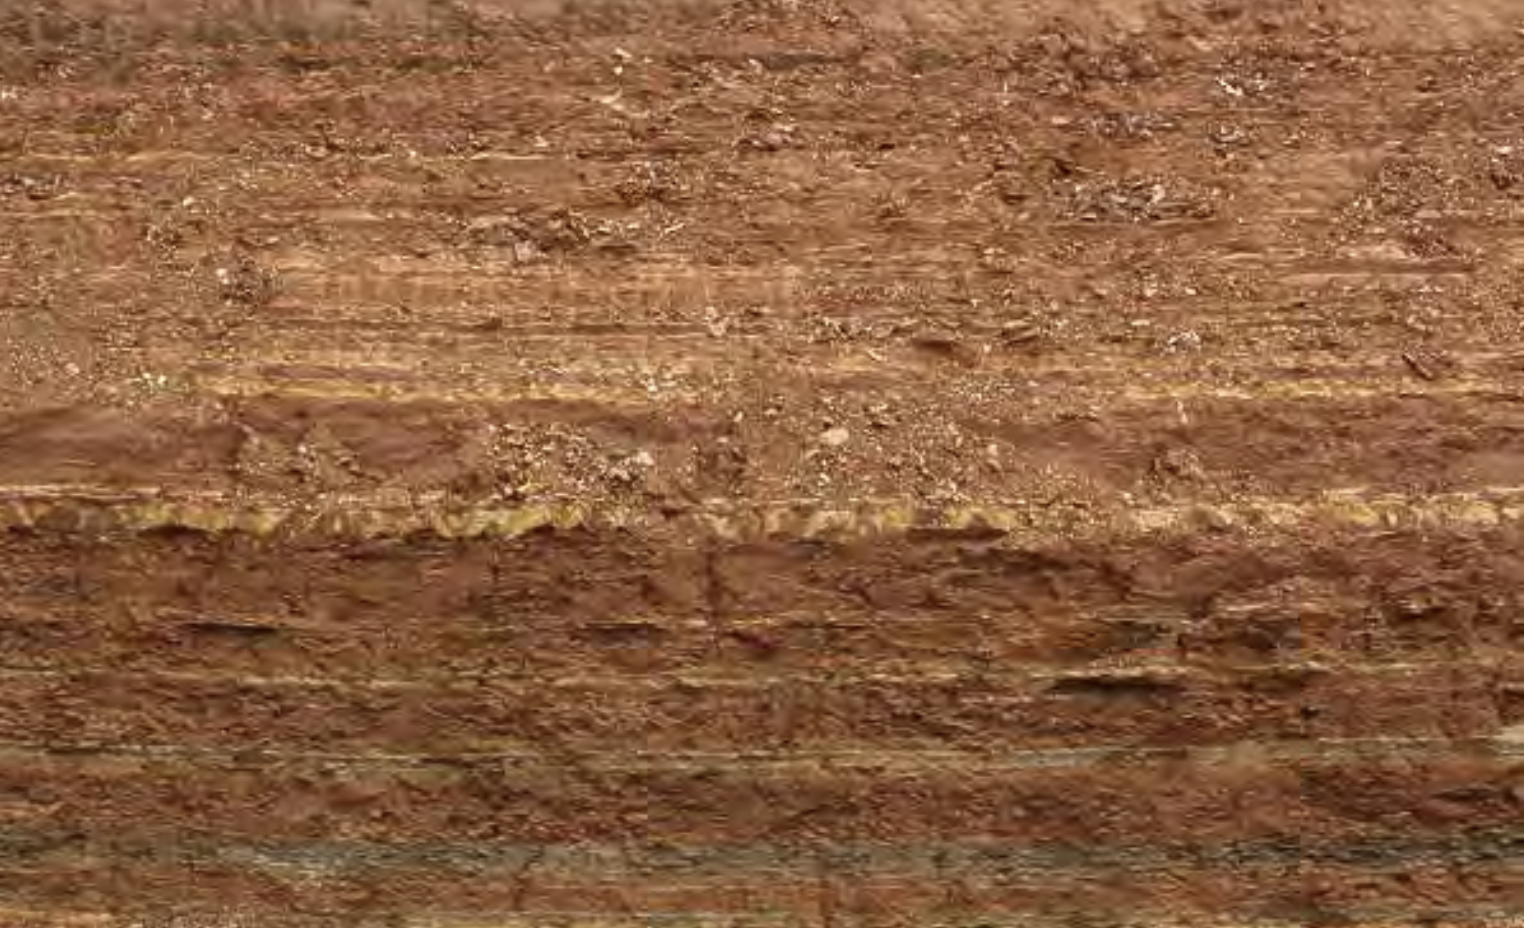
\includegraphics[width=0.8\textwidth]{layered-structure.png}
\end{frame}

\begin{frame}
    \frametitle{Модель плоской трещины}
    \centering
    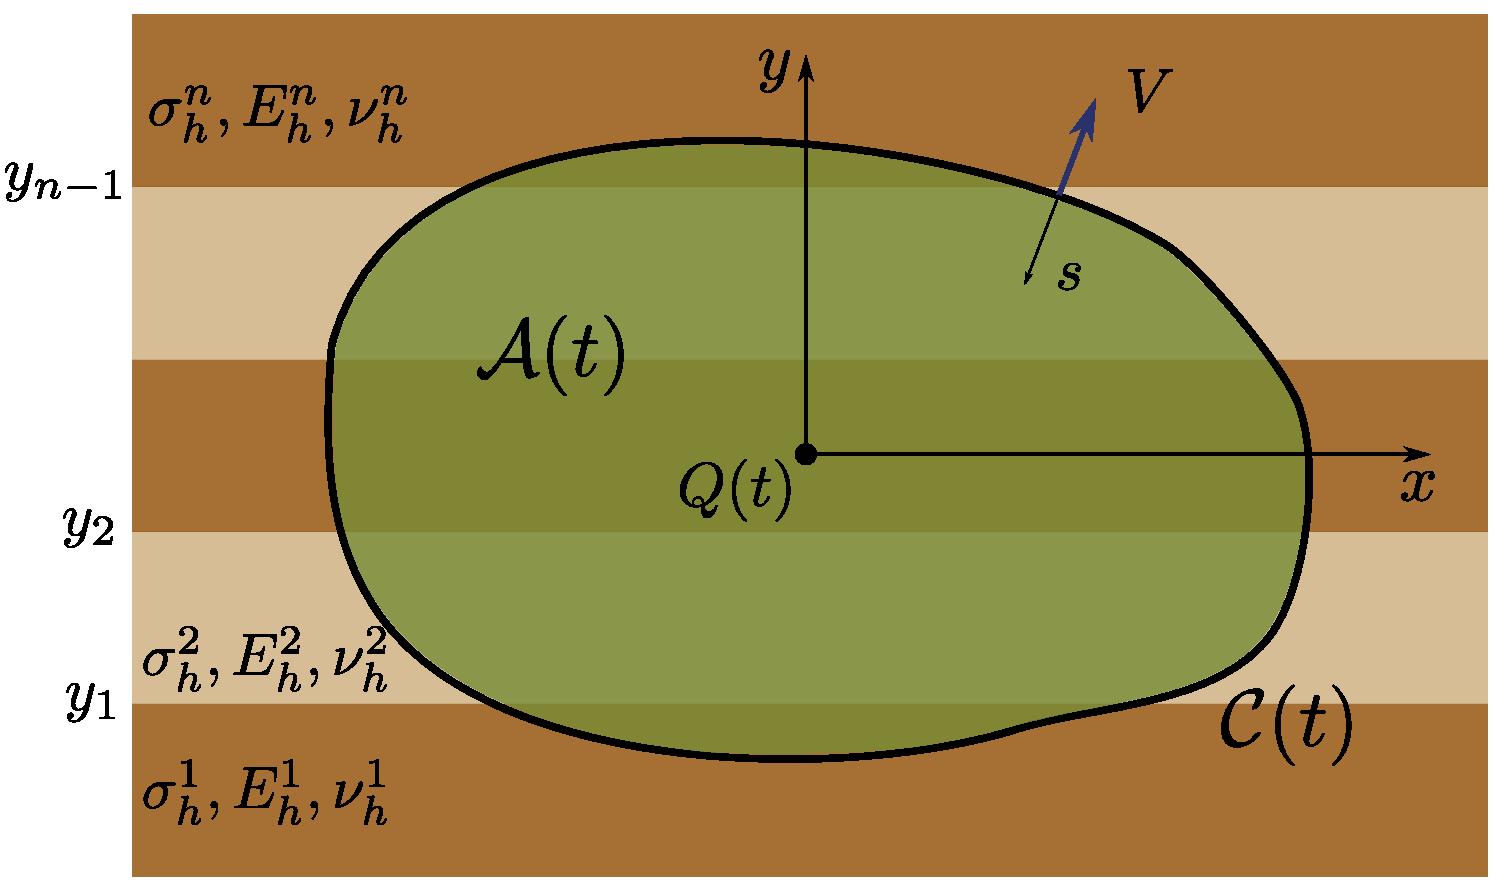
\includegraphics[width=0.8\textwidth]{fracture_scheme.pdf}
\end{frame}

\subsection{Определяющие уравнения}
\begin{frame}
    \frametitle{Закон сохранения массы}
    Уравнение неразрывности в приближении тонкого слоя для плоской трещины
    \begin{equation}
        \label{eq:conservation_law}
        \pd{w}{t} + \bigtriangledown \cdot q + \frac{2C_L}{\sqrt{t-t_0(x,\, y)}}  = Q(t) \delta(x,\,y),
    \end{equation}
    
    Используя закон Пуазейля $q  = -\frac{w^3}{12\mu} \bigtriangledown\! p$, получаем уравнение Рейнольдса
    \begin{equation}
        \label{eq:reynolds_equation}
        \pd{w}{t} - \text{div} \left( -\frac{w^3}{12\mu} \bigtriangledown \!p \right) + \frac{2C_L}{\sqrt{t-t_0(x,\, y)}}  = Q(t) \delta(x,\,y),
    \end{equation}
\end{frame}

\begin{frame}
    \frametitle{Уравнение упругости}
    Уравнение упругости связывает раскрытие трещины $w$ с давлением $p$
    \begin{equation}
        \label{eq:elasticity_equation}
        p(x,y,t) = \sigma_h(y) + \int\limits_{\mathcal{A}(t)} G(x,y;x',y')w(x',y',t) \dif x' \dif y',
    \end{equation} 

    В случае изотропной среды
    \begin{equation}
        \label{eq:elasticity_kernel}
        G(x,y;x',y') = - \frac{E'}{8\pi [(x\!-\!x')^2+(y\!-\!y')^2]^{3/2}}.
    \end{equation}
    $E' = E / (1-\nu^2)$, где $E$ -- модуль Юнга, $\nu$ -- коэффициент Пуассона.
\end{frame}

\subsection{Численная постановка}
\begin{frame}
    \frametitle{Численная постановка}
    Дискретизация уравнений \eqref{eq:reynolds_equation} и \eqref{eq:elasticity_equation} осуществляется с помощью метода разрывных смещений
    \begin{equation}
        \label{eq:piecewiece_approximation}
        \begin{split}
            w(x,y,t) &= \sum\limits_{i,j} w_{i,j}(t) H_{i,j}(x,y), \\
            p(x,y,t) &= \sum\limits_{i,j} p_{i,j}(t) H_{i,j}(x,y), \\
        \end{split}
    \end{equation}
    где 
    \begin{equation}
        \label{eq:heaviside_function}
        H_{i,j}(x,y) = \left\{
            \begin{array}{ll}
                1, & (x,y) \in \mathcal{A}_{i,j}, \\
                0, & (x,y) \notin \mathcal{A}_{i,j}.
            \end{array}\right.
    \end{equation}
\end{frame}

\begin{frame}
    \frametitle{Дискретизация определяющих уравнений}
    Путём явного интегрирования по элементу уравнение упругости \eqref{eq:elasticity_equation} сводится к
    \begin{equation}
        \label{eq:discrete_elasticity}
        p_{i,j}(t) = {\sigma_h}_{i,j} + \sum\limits_{k,l} C_{i,j;k,l} w_{k,l}(t),
    \end{equation}
    где $C_{i,j;k,l}$ -- матрица упругости. 
    \begin{equation}
        \label{eq:homogeneous_matrix}
        C_{i,j;k,l} = -\frac{E'}{8\pi} \left[\frac{\sqrt{(x_i\!-\!x)^2 + (y_j\!-\!y)^2}}{(x_i\!-\!x)(y_j\!-\!y)} \right]_{x=x_k-\Delta x/2, y=y_l-\Delta y/2}^{x=x_k+\Delta x/2, y=y_l+\Delta y/2},
    \end{equation}
    где $[f]_{x=x_1, y=y_1}^{x=x_2, y=y_2} = f(x_1,y_1) - f(x_1,y_2) - f(x_2,y_1) + f(x_2,y_2)$. Дискретизация уравнения Рейнольдса \eqref{eq:reynolds_equation} осуществляется путем интегрирования по времени и элементу.
\end{frame}


\section{Численное построение матрицы упругости}
\begin{frame}
    \frametitle{Уравнения равновесия и закон Гука}
    Определяющие уравнения упругой изотропной среды задаются формулами
    \begin{equation}
        \label{eq:equilibrium}
        \sigma_{ij,j} + f_j = 0,
    \end{equation}
    \begin{equation}		
        \sigma_{ij} = \lambda e_{kk}\delta_{ij} + 2G e_{ij},
        \label{eq:hooke_law}
    \end{equation}
    где $\lambda = \frac{E \nu}{(1+\nu)(1-2\nu)}$ и $ G = \frac{E}{2(1+\nu)} $.
    Отделяя производные по $y$ от производных по $x, z$
    \begin{equation}
        \label{eq:separate}
        \partial_{y} T = \mathbb{A}T + F,
    \end{equation}
    где
    \begin{equation}
        \label{eq:T}
        \begin{split}
            T &= \left[\sigma_{yy} \; \sigma_{xy} \; \sigma_{yz} \; u_{y} \; u_{x} \; u_{z}\right]^T, \\
            F &= \left[-f_y \; -f_x \; -f_z \; 0 \; 0 \; 0\right]^T,
        \end{split}
    \end{equation}
\end{frame}

\begin{frame}
    \frametitle{Дифференциальный оператор}
    \begin{equation*}
        \mathbb{A} = 
        \left[\begin{array}{cccccc}
            0                      & -\partial_x & -\partial_z & 0 & 0 & 0 \\
            -\frac{b}{a}\partial_x & 0           & 0 & 0 & \frac{b^2-a^2}{a}\partial_{xx} - \frac{f}{2}\partial_{zz} & \left( \frac{b^2-ab}{a} - \frac{f}{2} \right) \partial_{xz} \\
            -\frac{b}{a}\partial_z & 0           & 0 & 0 & \left( \frac{b^2-ab}{a} - \frac{f}{2} \right) \partial_{xz} & \frac{b^2-a^2}{a}\partial_{zz} - \frac{f}{2}\partial_{xx} \\
            \frac{1}{a}            & 0           & 0 & 0 & -\frac{b}{a}\partial_x & -\frac{b}{a}\partial_z \\
            0                      & \frac{2}{f} & 0 & -\partial_x & 0 & 0 \\
            0                      & 0           & \frac{2}{f} & -\partial_z & 0 & 0 
        \end{array}\right],
    \end{equation*}
    
    где используются константы
    \begin{align*}
        a   & = \lambda + 2G,                          & b   & = \lambda,                &     f & = 2G, \\
        l_2 & = \frac{\lambda + 3G}{\lambda + G},      & l_4 & = \frac{2G^2}{\lambda+G}, &   l_5 & = \frac{2G(\lambda + 2G)}{\lambda + G}, \\
        l_6 & = \frac{2G(2\lambda + 2G)}{\lambda + G}, & l_7 & = \frac{2\lambda G}{\lambda+G}
    \end{align*}
\end{frame}

\begin{frame}
    \frametitle{Постановка в Фурье образе}
    Применим двумерное преобразование Фурье по координатам $x$ и $z$
    \begin{equation}
        \label{eq:FT_system}
        \partial_y \hat{T} = \hat{\mathbb{A}} \hat{T} + \hat{F},
    \end{equation}
    где
    \begin{equation}
        \label{eq:FourierT}
        \begin{split}
            \hat{T} &= \left[\hat{\sigma}_{yy}/k \quad \hat{\tau}_s/k \quad \hat{u}_y \quad \hat{u}_s \quad  \hat{\tau}_t/k \quad  \hat{u}_t \right]^T, \\
            \hat{F} &= \left[-\hat{f}_y \; -\hat{f}_s \; 0 \; 0 \; -\hat{f}_t \; 0\right]^T,
        \end{split}
    \end{equation}

    \begin{equation}
        \label{eq:FourierA}
        \hat{\mathbb{A}} = 
        \left[\begin{array}{cccccc}
            0 & -k & 0 & 0 & 0 & 0 \\
            \frac{b}{a}k & 0 & 0 & -\frac{b^2-a^2}{a}k^2 & 0 & 0 \\
            \frac{1}{a} & 0 & 0 & -\frac{b}{a}k & 0 & 0 \\
            0 & \frac{2}{f} & k & 0 & 0 & 0 \\
            0 & 0 & 0 & 0 & 0 & \frac{f}{2}k \\
            0 & 0 & 0 & 0 & \frac{2}{f} & 0 
        \end{array}\right].
    \end{equation}
\end{frame}

\begin{frame}
    \frametitle{Введение псевдо-границы}
    \begin{minipage}[t]{0.47\linewidth}
        \footnotesize{Условие точечного разрыва смещений}
        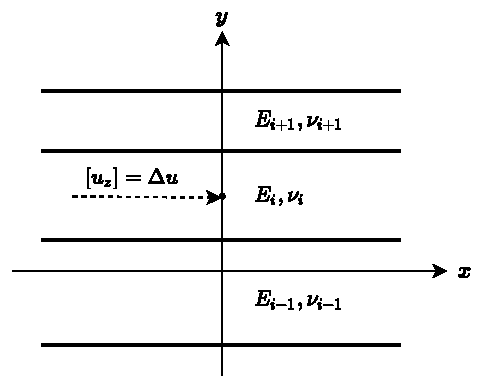
\includegraphics[width=\linewidth]{DD_point.pdf}
    \end{minipage}
    \hfill
    \begin{minipage}[t]{0.47\linewidth}
        \footnotesize{Введение дополнительной границы}
        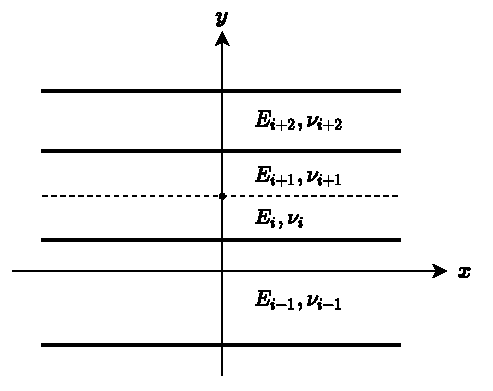
\includegraphics[width=\linewidth]{DD_point2.pdf}
    \end{minipage}
    Тогда $u_{z-0} - u_{z+0} = \Delta u$ может быть представлена в виде скачка смещения и напряжений на границе раздела слоев $\left[ \hat{T} \right] = \hat{T}(y-0) - \hat{T}(y+0)$.
\end{frame}

\begin{frame}
    \frametitle{Спектральные (свободные) коэффициенты}
    Система \eqref{eq:FT_system} является ОДУ и решение зависит от 6 свободных коэффициентов
    \begin{equation}
        \label{eq:fourier_solution}
        \left[
        \begin{array}{c}
            \hat{T}_s \\
            \hat{T}_t 
        \end{array}
        \right]
        =
        \left[
        \begin{array}{cc}
            Z_s & 0 \\
            0 & Z_t 
        \end{array}
        \right]
        \left[
        \begin{array}{c}
            A_s \\
            A_t 
        \end{array}
        \right]
    \end{equation}
    
    где используются обозначения
    \begin{equation}
        \label{eq:FourierSeparateT}
        \hat{T}_s = \left[\hat{\sigma}_{yy}/k \quad \hat{\tau}_s/k \quad \hat{u}_y \quad \hat{u}_s \right]^T, \qquad 
        \hat{T}_t = \left[ \hat{\tau}_t/k \quad  \hat{u}_t \right]^T.
    \end{equation}
\end{frame}

\begin{frame}
    \frametitle{Спектральные (свободные) коэффициенты}
    Связь между спектральными коэффициентами и значениями смещений и напряжений на границе слоя
    \begin{equation*}
        \left[
        \begin{array}{c}
        A^{j}_{1}(k) \\
        A^{j}_{2}(k)\\
        A^{j}_{3}(k) \\
        A^{j}_{4}(k)
        \end{array}
        \right]
        = \frac{1}{2l^j_5}
        \left[
        \begin{array}{cccc}
            -l^j_2 & 0 & l^j_5 & -l^j_4 \\
            -1 & 1 & f^j & -f^j \\
            l^j_2 & 0 & l^j_5 & l^j_4 \\
            -1 & -1 & -f^j & -f^j
        \end{array}
        \right]
        \left[
        \begin{array}{c}
        \hat{\sigma}^{j}_{yy}(y=y_j)/k \\
        \hat{\tau}^{j}_{s}(y=y_j)/k\\
        \hat{u}^{j}_{y}(y=y_j) \\
        \hat{u}^{j}_{s}(y=y_j) 
        \end{array}
        \right],
    \end{equation*}

    \begin{equation*}
        \left[
        \begin{array}{c}
            A^{j}_{5}(k) \\
            A^{j}_{6}(k)
        \end{array}
        \right]
        = \frac{1}{2l^j_5}
        \left[
        \begin{array}{cc}
            -\frac{1}{f^j} & \frac{1}{2} \\
            \frac{1}{f^j} & \frac{1}{2}
        \end{array}
        \right]
        \left[
        \begin{array}{c}
        \hat{\tau}^{j}_{t}(y=y_j)/k\\
        \hat{u}^{j}_{t}(y=y_j) 
        \end{array}
        \right].
    \end{equation*}
\end{frame}

\begin{frame}
    \frametitle{Связанные системы для граничных значений}
    Из этих соотношений можно составить уравнения для определения компонент вектора смещения и напряжений на границе раздела слоев
    \begin{equation}
        \label{eq:coupled_t-system}
        A_t^i \hat{\tau}_t^{i-1} + C_t^i \hat{\tau}_t^{i} + B_t^i \hat{\tau}_t^{i+1} = D_t^i,
    \end{equation}
    для t-системы и 
    \begin{equation}
        \label{eq:coupled_s-system}
        \textbf{A}_s^i \left[
            \begin{array}{c}
                \hat{\sigma}_{yy}^{i-1} \\
                \hat{\tau}_s^{i-1}
            \end{array}\right] +
        \textbf{C}_s^i \left[
            \begin{array}{c}
                \hat{\sigma}_{yy}^{i} \\
                \hat{\tau}_s^{i}
            \end{array}\right] + 
        \textbf{B}_s^i \left[
            \begin{array}{c}
                \hat{\sigma}_{yy}^{i+1} \\
                \hat{\tau}_s^{i+1}
            \end{array}\right]
        = \textbf{D}_s^i,
    \end{equation}
    для s-системы.
\end{frame}

\begin{frame}
    \frametitle{}
    Ядро $G(x,y;x',y')$ интегрального соотношения~\eqref{eq:elasticity_equation} для слоистой среды
    \begin{equation}
        G(x,y;x',y') = G_\text{hom}(x,y;x',y') + G'(x,y;x',y'),
    \end{equation} 
    где $G_\text{hom}(x,y;x',y')$ получается из \eqref{eq:elasticity_kernel} с учетом $E'=E'(y)$. Окончательно
    \begin{multline}
        \label{eq:fourier_sigmazz}
        \hat{\sigma}^j_{zz}(y)/k = f\frac{n^2}{k^2}e^{-ky}A^j_1(k)
        - \left(l_6\frac{n^2}{k^2}+l_7\frac{m^2}{k^2}-f\frac{n^2}{k^2}ky \right)e^{-ky}A^j_2(k) - \\
        - f\frac{n^2}{k^2}e^{ky}A^j_3(k)
        - \left(l_6\frac{n^2}{k^2}+l_7\frac{m^2}{k^2}+f\frac{n^2}{k^2}ky \right)e^{ky}A^j_4(k) - \\
        - f\frac{mn}{k^2}e^{-ky}A^j_5(k)
        - f\frac{mn}{k^2}e^{ky}A^j_6(k).
    \end{multline}
\end{frame}


\section{Верификация и численные расчеты}
\begin{frame}
    \frametitle{Радиальная трещина, $E_\text{b} = E_\text{m} = E_\text{t} = 10$~GPa, $\nu_\text{b} = \nu_\text{m} = \nu_\text{t} = 0.22$}
    \begin{minipage}[t]{0.4\linewidth}
        \includegraphics[width=\linewidth]{Homogeneous/Figures/1/width_29.pdf}
    \end{minipage}
    \hfill
    \begin{minipage}[t]{0.57\linewidth}
        \includegraphics[width=\linewidth]{Homogeneous/Figures/1/w_y_29.pdf}
    \end{minipage}
\end{frame}

\begin{frame}
    \frametitle{Пласт с жестким нижним слоем, $E_\text{b} = 50$~GPa, $E_\text{m} = E_\text{t} = 10$~GPa, $\nu_\text{b} = \nu_\text{m} = \nu_\text{t} = 0.22$}
    \begin{minipage}[t]{0.4\linewidth}
        \includegraphics[width=\linewidth]{Heterogeneous/Figures/1/width_29.pdf}
    \end{minipage}
    \hfill
    \begin{minipage}[t]{0.57\linewidth}
        \includegraphics[width=\linewidth]{Heterogeneous/Figures/1/w_y_29.pdf}
    \end{minipage}
\end{frame}

\begin{frame}
    \frametitle{Пласт с сильной неоднородностью, $E_\text{b} = 100$~GPa, $E_\text{m} = E_\text{t} = 10$~GPa, $\nu_\text{b} = \nu_\text{m} = \nu_\text{t} = 0.22$}
    \begin{minipage}[t]{0.4\linewidth}
        \includegraphics[width=\linewidth]{Heterogeneous/Figures/2/width_29.pdf}
    \end{minipage}
    \hfill
    \begin{minipage}[t]{0.57\linewidth}
        \includegraphics[width=\linewidth]{Heterogeneous/Figures/2/w_y_29.pdf}
    \end{minipage}
\end{frame}

\begin{frame}
    \frametitle{Пласт с сильной неоднородностью, $E_\text{m} = 10$~GPa, $E_\text{b} = E_\text{t} = 100$~GPa, $\nu_\text{b} = \nu_\text{m} = \nu_\text{t} = 0.22$}
    \begin{minipage}[t]{0.4\linewidth}
        \includegraphics[width=\linewidth]{Heterogeneous/Figures/3_3/width_29.pdf}
    \end{minipage}
    \hfill
    \begin{minipage}[t]{0.57\linewidth}
        \includegraphics[width=\linewidth]{Heterogeneous/Figures/3_3/w_y_29.pdf}
    \end{minipage}
\end{frame}

\begin{frame}
    \frametitle{$E_\text{b} = 20$~GPa, $E_\text{m} = E_\text{t} = 10$~GPa, $\nu_\text{b} = \nu_\text{m} = \nu_\text{t} = 0.22$, $\sigma_{h,\text{b}} = 30$~MPa, $\sigma_{h,\text{m}} = \sigma_{h,\text{t}} = 30.5$~MPa}
    \begin{minipage}[t]{0.4\linewidth}
        \includegraphics[width=\linewidth]{Heterogeneous/Figures/3/width_29.pdf}
    \end{minipage}
    \hfill
    \begin{minipage}[t]{0.57\linewidth}
        \includegraphics[width=\linewidth]{Heterogeneous/Figures/3/w_y_29.pdf}
    \end{minipage}
\end{frame}

\begin{frame}
    \frametitle{$E_\text{b} = 40$~GPa, $E_\text{m} = E_\text{t} = 10$~GPa, $\nu_\text{b} = \nu_\text{m} = \nu_\text{t} = 0.22$, $\sigma_{h,\text{b}} = 30$~MPa, $\sigma_{h,\text{m}} = \sigma_{h,\text{t}} = 30.5$~MPa}
    \begin{minipage}[t]{0.4\linewidth}
        \includegraphics[width=\linewidth]{Heterogeneous/Figures/3_2/width_29.pdf}
    \end{minipage}
    \hfill
    \begin{minipage}[t]{0.57\linewidth}
        \includegraphics[width=\linewidth]{Heterogeneous/Figures/3_2/w_y_29.pdf}
    \end{minipage}
\end{frame}

\begin{frame}
    \frametitle{Пласт с включением тонкого слоя, $d=10$~м. , $k=\frac{E_d}{E}=5$}
    \begin{minipage}[t]{0.4\linewidth}
        \includegraphics[width=\linewidth]{Heterogeneous/Figures/4/width_29.pdf}
    \end{minipage}
    \hfill
    \begin{minipage}[t]{0.57\linewidth}
        \includegraphics[width=\linewidth]{Heterogeneous/Figures/4/w_y_29.pdf}
    \end{minipage}
\end{frame}

\begin{frame}
    \frametitle{Пласт с включением двух тонких пропластков, $d=10$~м. , $k=\frac{E_d}{E}=5$}
    \begin{minipage}[t]{0.4\linewidth}
        \includegraphics[width=\linewidth]{Heterogeneous/Figures/5/width_29.pdf}
    \end{minipage}
    \hfill
    \begin{minipage}[t]{0.57\linewidth}
        \includegraphics[width=\linewidth]{Heterogeneous/Figures/5/w_y_29.pdf}
    \end{minipage}
\end{frame}